\documentclass{article}
\usepackage[utf8]{inputenc}
\usepackage{polski}
\usepackage{graphicx}
\usepackage{tikz}
\usepackage[export]{adjustbox}
\graphicspath{./images/}
\usepackage{listings}
\usepackage{xcolor}
\usepackage{amsmath}

\definecolor{codegreen}{rgb}{0,0.6,0}
\definecolor{codegray}{rgb}{0.5,0.5,0.5}
\definecolor{codepurple}{rgb}{0.58,0,0.82}
\definecolor{backcolour}{rgb}{0.95,0.95,0.92}

\lstdefinestyle{mystyle}{
    backgroundcolor=\color{backcolour},   
    commentstyle=\color{codegreen},
    keywordstyle=\color{magenta},
    numberstyle=\tiny\color{codegray},
    stringstyle=\color{codepurple},
    basicstyle=\ttfamily\footnotesize,
    breakatwhitespace=false,         
    breaklines=true,                 
    captionpos=b,                    
    keepspaces=true,                 
    numbers=left,                    
    numbersep=5pt,                  
    showspaces=false,                
    showstringspaces=false,
    showtabs=false,                  
    tabsize=2
}

\lstset{style=mystyle}

\title{Zadanie 1 - mnożenie macierzy za pomocą algorytmu klasycznego i Strassena}
\author{Mateusz Wejman, Andrzej Starzyk}
\date{March 2024}

\begin{document}

\maketitle

\section{Wykonanie}



\lstinputlisting[language=erlang]{code1.txt}
\lstinputlisting[language=erlang]{code2.txt}


\begin{figure}
    \centering
    \hspace*{-3cm}%
    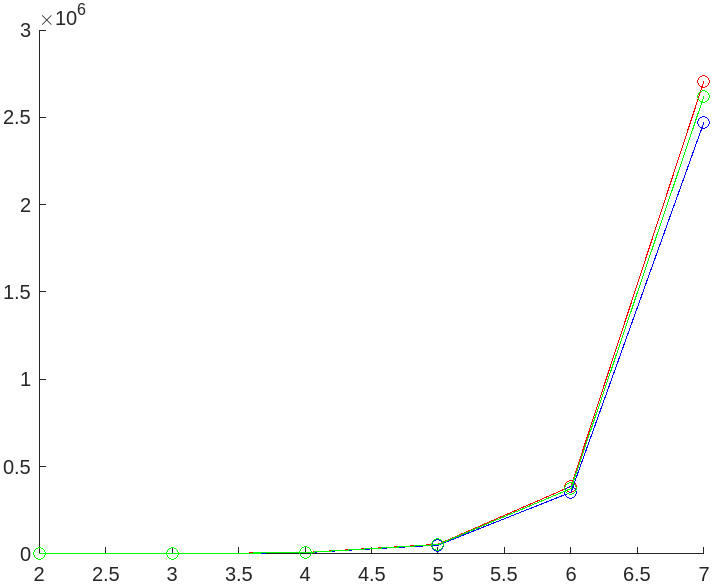
\includegraphics[width=1.5\textwidth]{images/img1.png}
    \caption{Ilość operacji zmiennoprzecinkowych w zależności od rozmiaru macierzy}
    \label{fig:my_label}
\end{figure}


\begin{figure}
    \centering
    \hspace*{-3cm}%
    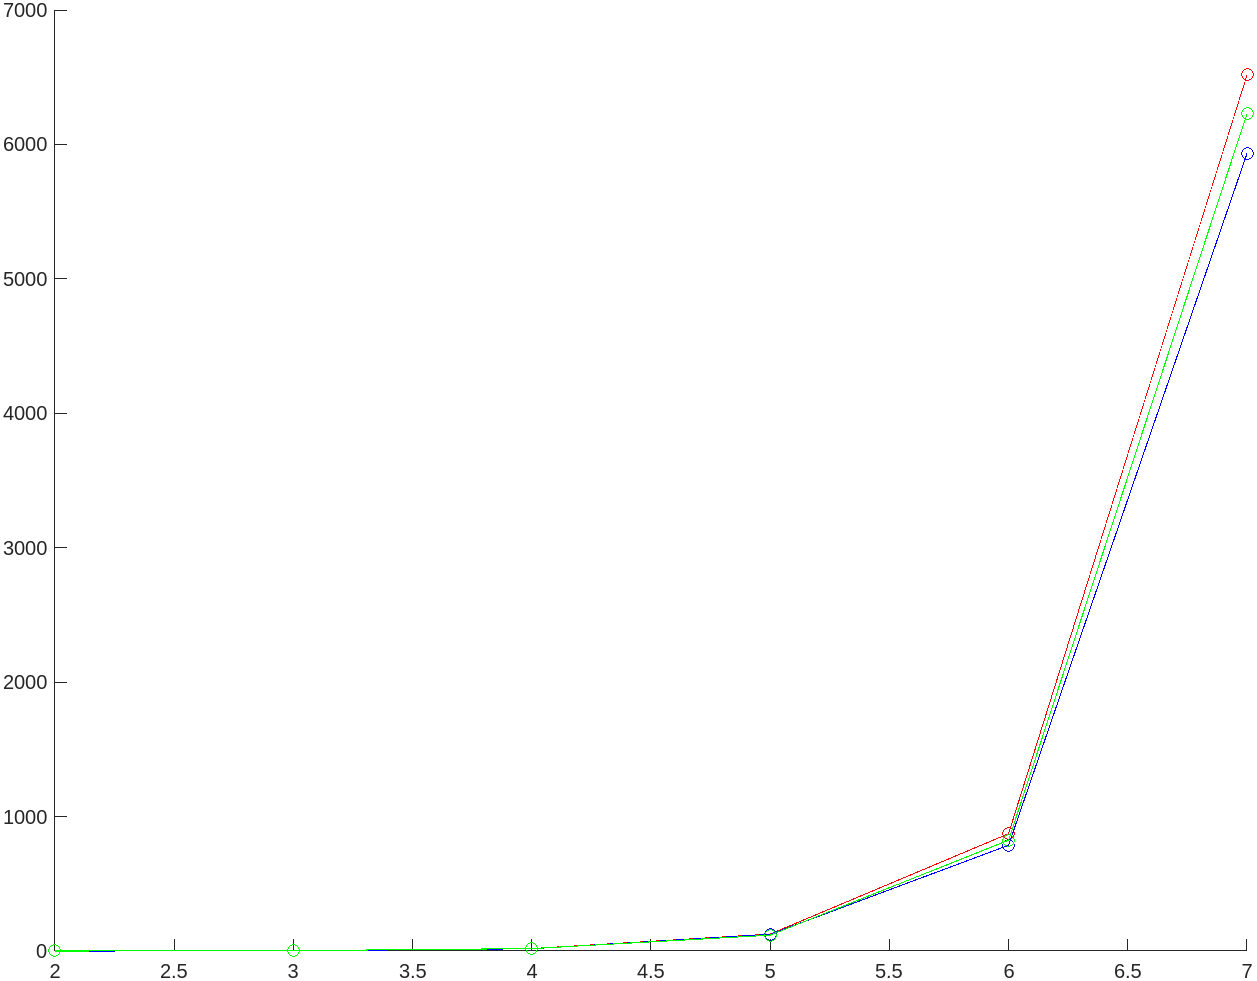
\includegraphics[width=1.5\textwidth]{images/img2.png}
    \caption{Czas wykonywania obliczeń (ms) w zależności od rozmiaru macierzy}
    \label{fig:my_label}
\end{figure}


\end{document}
